% Options for packages loaded elsewhere
% Options for packages loaded elsewhere
\PassOptionsToPackage{unicode}{hyperref}
\PassOptionsToPackage{hyphens}{url}
\PassOptionsToPackage{dvipsnames,svgnames,x11names}{xcolor}
%
\documentclass[
  letterpaper,
  DIV=11,
  numbers=noendperiod]{scrartcl}
\usepackage{xcolor}
\usepackage{amsmath,amssymb}
\setcounter{secnumdepth}{-\maxdimen} % remove section numbering
\usepackage{iftex}
\ifPDFTeX
  \usepackage[T1]{fontenc}
  \usepackage[utf8]{inputenc}
  \usepackage{textcomp} % provide euro and other symbols
\else % if luatex or xetex
  \usepackage{unicode-math} % this also loads fontspec
  \defaultfontfeatures{Scale=MatchLowercase}
  \defaultfontfeatures[\rmfamily]{Ligatures=TeX,Scale=1}
\fi
\usepackage{lmodern}
\ifPDFTeX\else
  % xetex/luatex font selection
\fi
% Use upquote if available, for straight quotes in verbatim environments
\IfFileExists{upquote.sty}{\usepackage{upquote}}{}
\IfFileExists{microtype.sty}{% use microtype if available
  \usepackage[]{microtype}
  \UseMicrotypeSet[protrusion]{basicmath} % disable protrusion for tt fonts
}{}
\makeatletter
\@ifundefined{KOMAClassName}{% if non-KOMA class
  \IfFileExists{parskip.sty}{%
    \usepackage{parskip}
  }{% else
    \setlength{\parindent}{0pt}
    \setlength{\parskip}{6pt plus 2pt minus 1pt}}
}{% if KOMA class
  \KOMAoptions{parskip=half}}
\makeatother
% Make \paragraph and \subparagraph free-standing
\makeatletter
\ifx\paragraph\undefined\else
  \let\oldparagraph\paragraph
  \renewcommand{\paragraph}{
    \@ifstar
      \xxxParagraphStar
      \xxxParagraphNoStar
  }
  \newcommand{\xxxParagraphStar}[1]{\oldparagraph*{#1}\mbox{}}
  \newcommand{\xxxParagraphNoStar}[1]{\oldparagraph{#1}\mbox{}}
\fi
\ifx\subparagraph\undefined\else
  \let\oldsubparagraph\subparagraph
  \renewcommand{\subparagraph}{
    \@ifstar
      \xxxSubParagraphStar
      \xxxSubParagraphNoStar
  }
  \newcommand{\xxxSubParagraphStar}[1]{\oldsubparagraph*{#1}\mbox{}}
  \newcommand{\xxxSubParagraphNoStar}[1]{\oldsubparagraph{#1}\mbox{}}
\fi
\makeatother

\usepackage{color}
\usepackage{fancyvrb}
\newcommand{\VerbBar}{|}
\newcommand{\VERB}{\Verb[commandchars=\\\{\}]}
\DefineVerbatimEnvironment{Highlighting}{Verbatim}{commandchars=\\\{\}}
% Add ',fontsize=\small' for more characters per line
\usepackage{framed}
\definecolor{shadecolor}{RGB}{241,243,245}
\newenvironment{Shaded}{\begin{snugshade}}{\end{snugshade}}
\newcommand{\AlertTok}[1]{\textcolor[rgb]{0.68,0.00,0.00}{#1}}
\newcommand{\AnnotationTok}[1]{\textcolor[rgb]{0.37,0.37,0.37}{#1}}
\newcommand{\AttributeTok}[1]{\textcolor[rgb]{0.40,0.45,0.13}{#1}}
\newcommand{\BaseNTok}[1]{\textcolor[rgb]{0.68,0.00,0.00}{#1}}
\newcommand{\BuiltInTok}[1]{\textcolor[rgb]{0.00,0.23,0.31}{#1}}
\newcommand{\CharTok}[1]{\textcolor[rgb]{0.13,0.47,0.30}{#1}}
\newcommand{\CommentTok}[1]{\textcolor[rgb]{0.37,0.37,0.37}{#1}}
\newcommand{\CommentVarTok}[1]{\textcolor[rgb]{0.37,0.37,0.37}{\textit{#1}}}
\newcommand{\ConstantTok}[1]{\textcolor[rgb]{0.56,0.35,0.01}{#1}}
\newcommand{\ControlFlowTok}[1]{\textcolor[rgb]{0.00,0.23,0.31}{\textbf{#1}}}
\newcommand{\DataTypeTok}[1]{\textcolor[rgb]{0.68,0.00,0.00}{#1}}
\newcommand{\DecValTok}[1]{\textcolor[rgb]{0.68,0.00,0.00}{#1}}
\newcommand{\DocumentationTok}[1]{\textcolor[rgb]{0.37,0.37,0.37}{\textit{#1}}}
\newcommand{\ErrorTok}[1]{\textcolor[rgb]{0.68,0.00,0.00}{#1}}
\newcommand{\ExtensionTok}[1]{\textcolor[rgb]{0.00,0.23,0.31}{#1}}
\newcommand{\FloatTok}[1]{\textcolor[rgb]{0.68,0.00,0.00}{#1}}
\newcommand{\FunctionTok}[1]{\textcolor[rgb]{0.28,0.35,0.67}{#1}}
\newcommand{\ImportTok}[1]{\textcolor[rgb]{0.00,0.46,0.62}{#1}}
\newcommand{\InformationTok}[1]{\textcolor[rgb]{0.37,0.37,0.37}{#1}}
\newcommand{\KeywordTok}[1]{\textcolor[rgb]{0.00,0.23,0.31}{\textbf{#1}}}
\newcommand{\NormalTok}[1]{\textcolor[rgb]{0.00,0.23,0.31}{#1}}
\newcommand{\OperatorTok}[1]{\textcolor[rgb]{0.37,0.37,0.37}{#1}}
\newcommand{\OtherTok}[1]{\textcolor[rgb]{0.00,0.23,0.31}{#1}}
\newcommand{\PreprocessorTok}[1]{\textcolor[rgb]{0.68,0.00,0.00}{#1}}
\newcommand{\RegionMarkerTok}[1]{\textcolor[rgb]{0.00,0.23,0.31}{#1}}
\newcommand{\SpecialCharTok}[1]{\textcolor[rgb]{0.37,0.37,0.37}{#1}}
\newcommand{\SpecialStringTok}[1]{\textcolor[rgb]{0.13,0.47,0.30}{#1}}
\newcommand{\StringTok}[1]{\textcolor[rgb]{0.13,0.47,0.30}{#1}}
\newcommand{\VariableTok}[1]{\textcolor[rgb]{0.07,0.07,0.07}{#1}}
\newcommand{\VerbatimStringTok}[1]{\textcolor[rgb]{0.13,0.47,0.30}{#1}}
\newcommand{\WarningTok}[1]{\textcolor[rgb]{0.37,0.37,0.37}{\textit{#1}}}

\usepackage{longtable,booktabs,array}
\newcounter{none} % for unnumbered tables
\usepackage{calc} % for calculating minipage widths
% Correct order of tables after \paragraph or \subparagraph
\usepackage{etoolbox}
\makeatletter
\patchcmd\longtable{\par}{\if@noskipsec\mbox{}\fi\par}{}{}
\makeatother
% Allow footnotes in longtable head/foot
\IfFileExists{footnotehyper.sty}{\usepackage{footnotehyper}}{\usepackage{footnote}}
\makesavenoteenv{longtable}
\usepackage{graphicx}
\makeatletter
\newsavebox\pandoc@box
\newcommand*\pandocbounded[1]{% scales image to fit in text height/width
  \sbox\pandoc@box{#1}%
  \Gscale@div\@tempa{\textheight}{\dimexpr\ht\pandoc@box+\dp\pandoc@box\relax}%
  \Gscale@div\@tempb{\linewidth}{\wd\pandoc@box}%
  \ifdim\@tempb\p@<\@tempa\p@\let\@tempa\@tempb\fi% select the smaller of both
  \ifdim\@tempa\p@<\p@\scalebox{\@tempa}{\usebox\pandoc@box}%
  \else\usebox{\pandoc@box}%
  \fi%
}
% Set default figure placement to htbp
\def\fps@figure{htbp}
\makeatother





\setlength{\emergencystretch}{3em} % prevent overfull lines

\providecommand{\tightlist}{%
  \setlength{\itemsep}{0pt}\setlength{\parskip}{0pt}}



 


\KOMAoption{captions}{tableheading}
\makeatletter
\@ifpackageloaded{caption}{}{\usepackage{caption}}
\AtBeginDocument{%
\ifdefined\contentsname
  \renewcommand*\contentsname{Table of contents}
\else
  \newcommand\contentsname{Table of contents}
\fi
\ifdefined\listfigurename
  \renewcommand*\listfigurename{List of Figures}
\else
  \newcommand\listfigurename{List of Figures}
\fi
\ifdefined\listtablename
  \renewcommand*\listtablename{List of Tables}
\else
  \newcommand\listtablename{List of Tables}
\fi
\ifdefined\figurename
  \renewcommand*\figurename{Figure}
\else
  \newcommand\figurename{Figure}
\fi
\ifdefined\tablename
  \renewcommand*\tablename{Table}
\else
  \newcommand\tablename{Table}
\fi
}
\@ifpackageloaded{float}{}{\usepackage{float}}
\floatstyle{ruled}
\@ifundefined{c@chapter}{\newfloat{codelisting}{h}{lop}}{\newfloat{codelisting}{h}{lop}[chapter]}
\floatname{codelisting}{Listing}
\newcommand*\listoflistings{\listof{codelisting}{List of Listings}}
\makeatother
\makeatletter
\makeatother
\makeatletter
\@ifpackageloaded{caption}{}{\usepackage{caption}}
\@ifpackageloaded{subcaption}{}{\usepackage{subcaption}}
\makeatother
\usepackage{bookmark}
\IfFileExists{xurl.sty}{\usepackage{xurl}}{} % add URL line breaks if available
\urlstyle{same}
% fallback for those not using the hyperref driver hyperxmp:
\makeatletter
\@ifundefined{xmpquote}{\newcommand{\xmpquote}[1]{#1}}{}
\makeatother
\hypersetup{
  pdftitle={Class 13: RNA Seq Analysis with DESeq2},
  colorlinks=true,
  linkcolor={blue},
  filecolor={Maroon},
  citecolor={Blue},
  urlcolor={Blue},
  pdfcreator={LaTeX via pandoc}}


\title{Class 13: RNA Seq Analysis with DESeq2}
\author{}
\date{}
\begin{document}
\maketitle


\subsection{Background}\label{background}

Today we will do our first RNASeq analysis of a dataset from a study of
a common synthetic glucocorticoid, called dexamethasone, on airway
smooth muscle cells.

\subsection{Data Import}\label{data-import}

There are two input CSV files to read, the first is so-called ``counts''
data the 2nd is metadata about the design of the experiment (i.e.~the
columns in''counts''):

\begin{Shaded}
\begin{Highlighting}[]
\NormalTok{counts }\OtherTok{\textless{}{-}} \FunctionTok{read.csv}\NormalTok{(}\StringTok{"airway\_scaledcounts.csv"}\NormalTok{, }\AttributeTok{row.names=}\DecValTok{1}\NormalTok{)}
\NormalTok{metadata }\OtherTok{\textless{}{-}} \FunctionTok{read.csv}\NormalTok{(}\StringTok{"airway\_metadata.csv"}\NormalTok{)}
\end{Highlighting}
\end{Shaded}

\begin{quote}
Q1. How many genes are in this dataset?
\end{quote}

38694 genes.

\begin{Shaded}
\begin{Highlighting}[]
\FunctionTok{nrow}\NormalTok{(counts)}
\end{Highlighting}
\end{Shaded}

\begin{verbatim}
[1] 38694
\end{verbatim}

\begin{quote}
Q2. How many `control' cell lines do we have?
\end{quote}

We have 4 control cell lines.

\begin{Shaded}
\begin{Highlighting}[]
\FunctionTok{sum}\NormalTok{(metadata}\SpecialCharTok{$}\NormalTok{dex }\SpecialCharTok{==} \StringTok{"control"}\NormalTok{)}
\end{Highlighting}
\end{Shaded}

\begin{verbatim}
[1] 4
\end{verbatim}

\begin{Shaded}
\begin{Highlighting}[]
\FunctionTok{table}\NormalTok{(metadata}\SpecialCharTok{$}\NormalTok{dex)}
\end{Highlighting}
\end{Shaded}

\begin{verbatim}

control treated 
      4       4 
\end{verbatim}

\begin{Shaded}
\begin{Highlighting}[]
\NormalTok{control }\OtherTok{\textless{}{-}}\NormalTok{ metadata[metadata[,}\StringTok{"dex"}\NormalTok{]}\SpecialCharTok{==}\StringTok{"control"}\NormalTok{,]}
\NormalTok{control.counts }\OtherTok{\textless{}{-}}\NormalTok{ counts[ ,control}\SpecialCharTok{$}\NormalTok{id]}
\NormalTok{control.mean }\OtherTok{\textless{}{-}} \FunctionTok{rowSums}\NormalTok{( control.counts )}\SpecialCharTok{/}\DecValTok{4} 
\FunctionTok{head}\NormalTok{(control.mean)}
\end{Highlighting}
\end{Shaded}

\begin{verbatim}
ENSG00000000003 ENSG00000000005 ENSG00000000419 ENSG00000000457 ENSG00000000460 
         900.75            0.00          520.50          339.75           97.25 
ENSG00000000938 
           0.75 
\end{verbatim}

\begin{Shaded}
\begin{Highlighting}[]
\FunctionTok{library}\NormalTok{(dplyr)}
\end{Highlighting}
\end{Shaded}

\begin{verbatim}

Attaching package: 'dplyr'
\end{verbatim}

\begin{verbatim}
The following objects are masked from 'package:stats':

    filter, lag
\end{verbatim}

\begin{verbatim}
The following objects are masked from 'package:base':

    intersect, setdiff, setequal, union
\end{verbatim}

\begin{Shaded}
\begin{Highlighting}[]
\NormalTok{control }\OtherTok{\textless{}{-}}\NormalTok{ metadata }\SpecialCharTok{\%\textgreater{}\%} \FunctionTok{filter}\NormalTok{(dex}\SpecialCharTok{==}\StringTok{"control"}\NormalTok{)}
\NormalTok{control.counts }\OtherTok{\textless{}{-}}\NormalTok{ counts }\SpecialCharTok{\%\textgreater{}\%} \FunctionTok{select}\NormalTok{(control}\SpecialCharTok{$}\NormalTok{id) }
\NormalTok{control.mean }\OtherTok{\textless{}{-}} \FunctionTok{rowSums}\NormalTok{(control.counts)}\SpecialCharTok{/}\DecValTok{4}
\FunctionTok{head}\NormalTok{(control.mean)}
\end{Highlighting}
\end{Shaded}

\begin{verbatim}
ENSG00000000003 ENSG00000000005 ENSG00000000419 ENSG00000000457 ENSG00000000460 
         900.75            0.00          520.50          339.75           97.25 
ENSG00000000938 
           0.75 
\end{verbatim}

\begin{Shaded}
\begin{Highlighting}[]
\FunctionTok{library}\NormalTok{(dplyr)}
\NormalTok{control }\OtherTok{\textless{}{-}}\NormalTok{ metadata }\SpecialCharTok{\%\textgreater{}\%} \FunctionTok{filter}\NormalTok{(dex}\SpecialCharTok{==}\StringTok{"control"}\NormalTok{)}
\NormalTok{control.counts }\OtherTok{\textless{}{-}}\NormalTok{ counts }\SpecialCharTok{\%\textgreater{}\%} \FunctionTok{select}\NormalTok{(control}\SpecialCharTok{$}\NormalTok{id) }
\NormalTok{control.mean }\OtherTok{\textless{}{-}} \FunctionTok{rowMeans}\NormalTok{(control.counts)}
\FunctionTok{head}\NormalTok{(control.mean)}
\end{Highlighting}
\end{Shaded}

\begin{verbatim}
ENSG00000000003 ENSG00000000005 ENSG00000000419 ENSG00000000457 ENSG00000000460 
         900.75            0.00          520.50          339.75           97.25 
ENSG00000000938 
           0.75 
\end{verbatim}

\begin{quote}
Q3. How would you make the above code in either approach more robust? Is
there a function that could help here?
\end{quote}

You can make the above code in either approach more robust by using
rowSums or rowMeans, where instead of doing control.mean \textless-
rowSums(control.counts)/4, you can do control.mean \textless-
rowMeans(control.counts).

\begin{quote}
Q4. Follow the same procedure for the treated samples (i.e.~calculate
the mean per gene across drug treated samples and assign to a labeled
vector called treated.mean)
\end{quote}

\begin{Shaded}
\begin{Highlighting}[]
\NormalTok{treated }\OtherTok{\textless{}{-}}\NormalTok{ metadata[metadata[,}\StringTok{"dex"}\NormalTok{]}\SpecialCharTok{==}\StringTok{"treated"}\NormalTok{,]}
\NormalTok{treated.mean }\OtherTok{\textless{}{-}} \FunctionTok{rowMeans}\NormalTok{( counts[ ,treated}\SpecialCharTok{$}\NormalTok{id] )}
\FunctionTok{head}\NormalTok{(treated.mean)}
\end{Highlighting}
\end{Shaded}

\begin{verbatim}
ENSG00000000003 ENSG00000000005 ENSG00000000419 ENSG00000000457 ENSG00000000460 
         658.00            0.00          546.00          316.50           78.75 
ENSG00000000938 
           0.00 
\end{verbatim}

\subsection{Analysis}\label{analysis}

\begin{Shaded}
\begin{Highlighting}[]
\FunctionTok{head}\NormalTok{(counts)}
\end{Highlighting}
\end{Shaded}

\begin{verbatim}
                SRR1039508 SRR1039509 SRR1039512 SRR1039513 SRR1039516
ENSG00000000003        723        486        904        445       1170
ENSG00000000005          0          0          0          0          0
ENSG00000000419        467        523        616        371        582
ENSG00000000457        347        258        364        237        318
ENSG00000000460         96         81         73         66        118
ENSG00000000938          0          0          1          0          2
                SRR1039517 SRR1039520 SRR1039521
ENSG00000000003       1097        806        604
ENSG00000000005          0          0          0
ENSG00000000419        781        417        509
ENSG00000000457        447        330        324
ENSG00000000460         94        102         74
ENSG00000000938          0          0          0
\end{verbatim}

\subsubsection{Our Plan}\label{our-plan}

We want to control our ``control'' vs ``treated'' (i.e.~no drug vs drug
experiments). We can calculate the mean count value for every gene
(rows) in all 4 ``control'' experiments and compare it to the mean
``count'' value in all ``treated'' experiments (i.e.~columns).

\begin{enumerate}
\def\labelenumi{\arabic{enumi}.}
\tightlist
\item
  Extract all ``control'' columns
\item
  Calculate the mean for each row (gene) of these columns
\item
  Do the same for ``treated'' to get a \texttt{treated.mean}
\end{enumerate}

\begin{Shaded}
\begin{Highlighting}[]
\NormalTok{metadata}\SpecialCharTok{$}\NormalTok{dex }\SpecialCharTok{==} \StringTok{"control"}
\end{Highlighting}
\end{Shaded}

\begin{verbatim}
[1]  TRUE FALSE  TRUE FALSE  TRUE FALSE  TRUE FALSE
\end{verbatim}

\begin{Shaded}
\begin{Highlighting}[]
\NormalTok{control.inds }\OtherTok{\textless{}{-}}\NormalTok{ metadata}\SpecialCharTok{$}\NormalTok{dex }\SpecialCharTok{==} \StringTok{"control"}
\end{Highlighting}
\end{Shaded}

\begin{Shaded}
\begin{Highlighting}[]
\NormalTok{control.counts }\OtherTok{\textless{}{-}}\NormalTok{ counts[,control.inds]}
\FunctionTok{dim}\NormalTok{(control.counts)}
\end{Highlighting}
\end{Shaded}

\begin{verbatim}
[1] 38694     4
\end{verbatim}

\begin{Shaded}
\begin{Highlighting}[]
\FunctionTok{head}\NormalTok{(control.counts)}
\end{Highlighting}
\end{Shaded}

\begin{verbatim}
                SRR1039508 SRR1039512 SRR1039516 SRR1039520
ENSG00000000003        723        904       1170        806
ENSG00000000005          0          0          0          0
ENSG00000000419        467        616        582        417
ENSG00000000457        347        364        318        330
ENSG00000000460         96         73        118        102
ENSG00000000938          0          1          2          0
\end{verbatim}

\begin{Shaded}
\begin{Highlighting}[]
\FunctionTok{library}\NormalTok{(dplyr)}

\NormalTok{control.mean }\OtherTok{\textless{}{-}} \FunctionTok{rowMeans}\NormalTok{(control.counts)}
\end{Highlighting}
\end{Shaded}

\begin{Shaded}
\begin{Highlighting}[]
\NormalTok{treated.mean }\OtherTok{\textless{}{-}}\FunctionTok{rowMeans}\NormalTok{(counts[,metadata}\SpecialCharTok{$}\NormalTok{dex}\SpecialCharTok{==}\StringTok{"treated"}\NormalTok{])}
\FunctionTok{head}\NormalTok{(treated.mean)}
\end{Highlighting}
\end{Shaded}

\begin{verbatim}
ENSG00000000003 ENSG00000000005 ENSG00000000419 ENSG00000000457 ENSG00000000460 
         658.00            0.00          546.00          316.50           78.75 
ENSG00000000938 
           0.00 
\end{verbatim}

For easy book-keeping lets store these two mean values together in one
data.frame called \texttt{mycounts}

\begin{Shaded}
\begin{Highlighting}[]
\NormalTok{meancounts }\OtherTok{\textless{}{-}} \FunctionTok{data.frame}\NormalTok{(control.mean, treated.mean)}
\end{Highlighting}
\end{Shaded}

\begin{quote}
Q5 (a). Create a scatter plot showing the mean of the treated samples
against the mean of the control samples. Your plot should look something
like the following.
\end{quote}

\begin{Shaded}
\begin{Highlighting}[]
\FunctionTok{plot}\NormalTok{(meancounts)}
\end{Highlighting}
\end{Shaded}

\pandocbounded{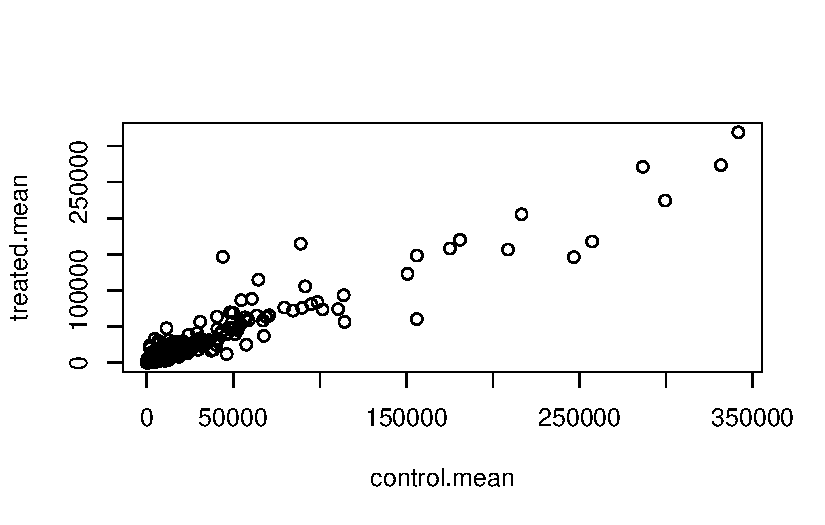
\includegraphics[keepaspectratio]{CLASS-13-WK-6-THURSDAY_files/figure-pdf/unnamed-chunk-17-1.pdf}}

\begin{Shaded}
\begin{Highlighting}[]
\FunctionTok{plot}\NormalTok{(meancounts[,}\DecValTok{1}\NormalTok{],meancounts[,}\DecValTok{2}\NormalTok{], }\AttributeTok{xlab=}\StringTok{"Control"}\NormalTok{, }\AttributeTok{ylab=}\StringTok{"Treated"}\NormalTok{)}
\end{Highlighting}
\end{Shaded}

\pandocbounded{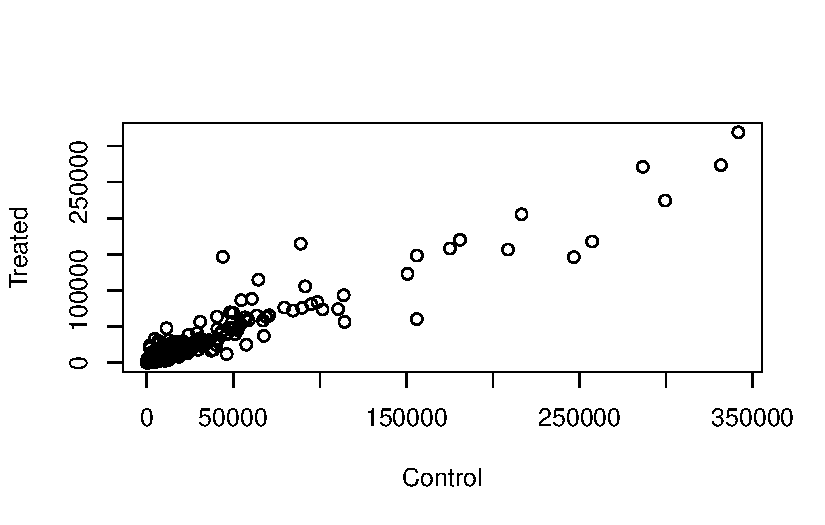
\includegraphics[keepaspectratio]{CLASS-13-WK-6-THURSDAY_files/figure-pdf/unnamed-chunk-18-1.pdf}}

\begin{quote}
Q5 (b).You could also use the ggplot2 package to make this figure
producing the plot below. What geom\_?() function would you use for this
plot?
\end{quote}

You would use geom\_point.

\begin{Shaded}
\begin{Highlighting}[]
\FunctionTok{library}\NormalTok{(ggplot2)}

\FunctionTok{ggplot}\NormalTok{(meancounts) }\SpecialCharTok{+} \FunctionTok{aes}\NormalTok{(control.mean, treated.mean) }\SpecialCharTok{+} \FunctionTok{geom\_point}\NormalTok{()}
\end{Highlighting}
\end{Shaded}

\pandocbounded{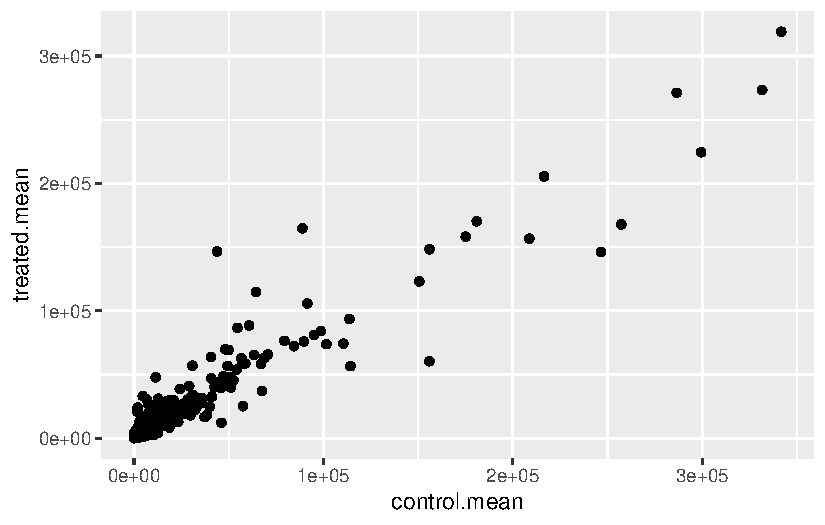
\includegraphics[keepaspectratio]{CLASS-13-WK-6-THURSDAY_files/figure-pdf/unnamed-chunk-19-1.pdf}}

\begin{quote}
Q. Re-draw or re-plot these on a log-log axis scale.
\end{quote}

\begin{quote}
Q6. Try plotting both axes on a log scale. What is the argument to
plot() that allows you to do this?
\end{quote}

The argument that allows you to do this is `log' or specifically
log=``xy''.

\begin{Shaded}
\begin{Highlighting}[]
\FunctionTok{plot}\NormalTok{(meancounts, }\AttributeTok{log=}\StringTok{"xy"}\NormalTok{)}
\end{Highlighting}
\end{Shaded}

\begin{verbatim}
Warning in xy.coords(x, y, xlabel, ylabel, log): 15032 x values <= 0 omitted
from logarithmic plot
\end{verbatim}

\begin{verbatim}
Warning in xy.coords(x, y, xlabel, ylabel, log): 15281 y values <= 0 omitted
from logarithmic plot
\end{verbatim}

\pandocbounded{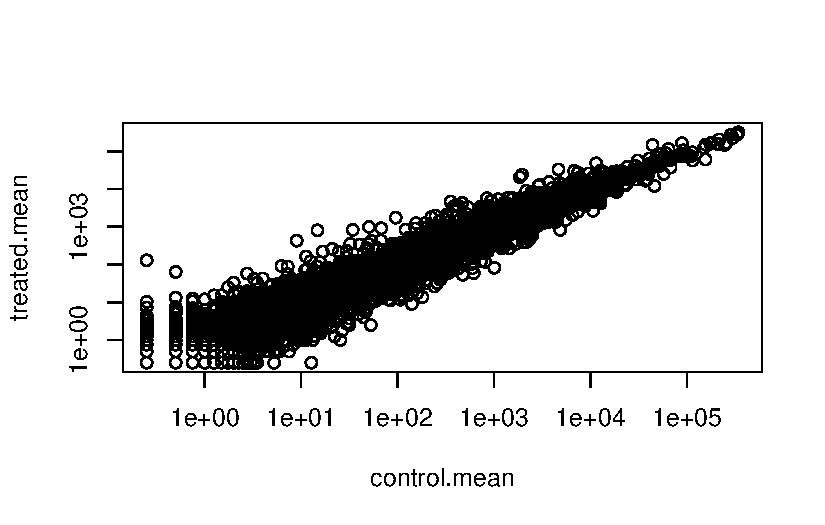
\includegraphics[keepaspectratio]{CLASS-13-WK-6-THURSDAY_files/figure-pdf/unnamed-chunk-20-1.pdf}}

We can compare the mean values of treated and control in terms of ``log
fold change values''. Typically we use log2 units of
``treated/control'':

\begin{Shaded}
\begin{Highlighting}[]
\CommentTok{\# No change = 0}
\FunctionTok{log2}\NormalTok{(}\DecValTok{20}\SpecialCharTok{/}\DecValTok{20}\NormalTok{)}
\end{Highlighting}
\end{Shaded}

\begin{verbatim}
[1] 0
\end{verbatim}

\begin{Shaded}
\begin{Highlighting}[]
\CommentTok{\# Up regulated = 1}
\FunctionTok{log2}\NormalTok{(}\DecValTok{40}\SpecialCharTok{/}\DecValTok{20}\NormalTok{)}
\end{Highlighting}
\end{Shaded}

\begin{verbatim}
[1] 1
\end{verbatim}

\begin{Shaded}
\begin{Highlighting}[]
\CommentTok{\# Down regulation, below the sloped line}
\FunctionTok{log2}\NormalTok{(}\DecValTok{20}\SpecialCharTok{/}\DecValTok{40}\NormalTok{)}
\end{Highlighting}
\end{Shaded}

\begin{verbatim}
[1] -1
\end{verbatim}

Let's add our Log2 Fold Change \texttt{log2fc} values to our
\texttt{meancounts} data frame.

\begin{Shaded}
\begin{Highlighting}[]
\NormalTok{meancounts}\SpecialCharTok{$}\NormalTok{log2fc }\OtherTok{\textless{}{-}}\FunctionTok{log2}\NormalTok{(meancounts}\SpecialCharTok{$}\NormalTok{treated.mean}\SpecialCharTok{/}\NormalTok{meancounts}\SpecialCharTok{$}\NormalTok{control.mean)}
\end{Highlighting}
\end{Shaded}

\begin{Shaded}
\begin{Highlighting}[]
\FunctionTok{head}\NormalTok{(meancounts)}
\end{Highlighting}
\end{Shaded}

\begin{verbatim}
                control.mean treated.mean      log2fc
ENSG00000000003       900.75       658.00 -0.45303916
ENSG00000000005         0.00         0.00         NaN
ENSG00000000419       520.50       546.00  0.06900279
ENSG00000000457       339.75       316.50 -0.10226805
ENSG00000000460        97.25        78.75 -0.30441833
ENSG00000000938         0.75         0.00        -Inf
\end{verbatim}

A common threshold for calling a gene ``up regulated'' is a log2fc value
of +2. For ``down regulated'' it is -2.

First filter out zero count genes - as we can't say anything about them
if we don't have any count data for them.

\begin{Shaded}
\begin{Highlighting}[]
\NormalTok{meancounts}\SpecialCharTok{$}\NormalTok{log2fc }\OtherTok{\textless{}{-}} \FunctionTok{log2}\NormalTok{(meancounts[,}\StringTok{"treated.mean"}\NormalTok{]}\SpecialCharTok{/}\NormalTok{meancounts[,}\StringTok{"control.mean"}\NormalTok{])}
\FunctionTok{head}\NormalTok{(meancounts)}
\end{Highlighting}
\end{Shaded}

\begin{verbatim}
                control.mean treated.mean      log2fc
ENSG00000000003       900.75       658.00 -0.45303916
ENSG00000000005         0.00         0.00         NaN
ENSG00000000419       520.50       546.00  0.06900279
ENSG00000000457       339.75       316.50 -0.10226805
ENSG00000000460        97.25        78.75 -0.30441833
ENSG00000000938         0.75         0.00        -Inf
\end{verbatim}

\begin{Shaded}
\begin{Highlighting}[]
\NormalTok{zero.vals }\OtherTok{\textless{}{-}} \FunctionTok{which}\NormalTok{(meancounts[,}\DecValTok{1}\SpecialCharTok{:}\DecValTok{2}\NormalTok{]}\SpecialCharTok{==}\DecValTok{0}\NormalTok{, }\AttributeTok{arr.ind=}\ConstantTok{TRUE}\NormalTok{)}

\NormalTok{to.rm }\OtherTok{\textless{}{-}} \FunctionTok{unique}\NormalTok{(zero.vals[,}\DecValTok{1}\NormalTok{])}
\NormalTok{mycounts }\OtherTok{\textless{}{-}}\NormalTok{ meancounts[}\SpecialCharTok{{-}}\NormalTok{to.rm,]}
\FunctionTok{head}\NormalTok{(mycounts)}
\end{Highlighting}
\end{Shaded}

\begin{verbatim}
                control.mean treated.mean      log2fc
ENSG00000000003       900.75       658.00 -0.45303916
ENSG00000000419       520.50       546.00  0.06900279
ENSG00000000457       339.75       316.50 -0.10226805
ENSG00000000460        97.25        78.75 -0.30441833
ENSG00000000971      5219.00      6687.50  0.35769358
ENSG00000001036      2327.00      1785.75 -0.38194109
\end{verbatim}

\begin{quote}
Q7. What is the purpose of the arr.ind argument in the which() function
call above? Why would we then take the first column of the output and
need to call the unique() function?
\end{quote}

The arr.ind=TRUE argument is a logical that would help give the specific
rows and columns that are `true' values, indicating the genes and
samples that have 0 counts. We would then take the first column of the
output and call the unique() function as it removes duplicate rows (the
genes) so they won't be counted twice.

\begin{quote}
Q8. Using the up.ind vector above can you determine how many up
regulated genes we have at the greater than 2 fc level?
\end{quote}

There are 250 up regulated genes at the greater than 2 fc level.

\begin{Shaded}
\begin{Highlighting}[]
\NormalTok{up.ind }\OtherTok{\textless{}{-}}\NormalTok{ mycounts}\SpecialCharTok{$}\NormalTok{log2fc }\SpecialCharTok{\textgreater{}} \DecValTok{2}
\NormalTok{down.ind }\OtherTok{\textless{}{-}}\NormalTok{ mycounts}\SpecialCharTok{$}\NormalTok{log2fc }\SpecialCharTok{\textless{}}\NormalTok{ (}\SpecialCharTok{{-}}\DecValTok{2}\NormalTok{)}
\FunctionTok{sum}\NormalTok{(up.ind)}
\end{Highlighting}
\end{Shaded}

\begin{verbatim}
[1] 250
\end{verbatim}

\begin{quote}
Q9. Using the down.ind vector above can you determine how many down
regulated genes we have at the greater than 2 fc level?
\end{quote}

There are 367 down regulated genes that are at the greater than 2 fc
level.

\begin{Shaded}
\begin{Highlighting}[]
\NormalTok{up.ind }\OtherTok{\textless{}{-}}\NormalTok{ mycounts}\SpecialCharTok{$}\NormalTok{log2fc }\SpecialCharTok{\textgreater{}} \DecValTok{2}
\NormalTok{down.ind }\OtherTok{\textless{}{-}}\NormalTok{ mycounts}\SpecialCharTok{$}\NormalTok{log2fc }\SpecialCharTok{\textless{}}\NormalTok{ (}\SpecialCharTok{{-}}\DecValTok{2}\NormalTok{)}
\FunctionTok{sum}\NormalTok{(down.ind)}
\end{Highlighting}
\end{Shaded}

\begin{verbatim}
[1] 367
\end{verbatim}

\begin{quote}
Q. How many genes are ``up regulated'' at +2 or above?
\end{quote}

314 genes up regulated at either +2 or above.

\begin{Shaded}
\begin{Highlighting}[]
\FunctionTok{sum}\NormalTok{(mycounts}\SpecialCharTok{$}\NormalTok{log2fc }\SpecialCharTok{\textgreater{}=} \DecValTok{2}\NormalTok{)}
\end{Highlighting}
\end{Shaded}

\begin{verbatim}
[1] 314
\end{verbatim}

\begin{quote}
Q10. Do you trust these results? Why or why not?
\end{quote}

No we do not trust these results as there are 30,000 genes, and also as
we're only relying on fold change and we haven't done any statistical
tests like P-value testing to see if these differences are significant
or not.

\#\#DESeq2 Analysis

Let's do this properly and put a P-value on these differences to keep
our inner stats nerd happy!

\begin{Shaded}
\begin{Highlighting}[]
\FunctionTok{library}\NormalTok{(DESeq2)}
\end{Highlighting}
\end{Shaded}

\begin{verbatim}
Loading required package: S4Vectors
\end{verbatim}

\begin{verbatim}
Loading required package: stats4
\end{verbatim}

\begin{verbatim}
Loading required package: BiocGenerics
\end{verbatim}

\begin{verbatim}
Loading required package: generics
\end{verbatim}

\begin{verbatim}

Attaching package: 'generics'
\end{verbatim}

\begin{verbatim}
The following object is masked from 'package:dplyr':

    explain
\end{verbatim}

\begin{verbatim}
The following objects are masked from 'package:base':

    as.difftime, as.factor, as.ordered, intersect, is.element, setdiff,
    setequal, union
\end{verbatim}

\begin{verbatim}

Attaching package: 'BiocGenerics'
\end{verbatim}

\begin{verbatim}
The following object is masked from 'package:dplyr':

    combine
\end{verbatim}

\begin{verbatim}
The following objects are masked from 'package:stats':

    IQR, mad, sd, var, xtabs
\end{verbatim}

\begin{verbatim}
The following objects are masked from 'package:base':

    anyDuplicated, aperm, append, as.data.frame, basename, cbind,
    colnames, dirname, do.call, duplicated, eval, evalq, Filter, Find,
    get, grep, grepl, is.unsorted, lapply, Map, mapply, match, mget,
    order, paste, pmax, pmax.int, pmin, pmin.int, Position, rank,
    rbind, Reduce, rownames, sapply, saveRDS, table, tapply, unique,
    unsplit, which.max, which.min
\end{verbatim}

\begin{verbatim}

Attaching package: 'S4Vectors'
\end{verbatim}

\begin{verbatim}
The following objects are masked from 'package:dplyr':

    first, rename
\end{verbatim}

\begin{verbatim}
The following object is masked from 'package:utils':

    findMatches
\end{verbatim}

\begin{verbatim}
The following objects are masked from 'package:base':

    expand.grid, I, unname
\end{verbatim}

\begin{verbatim}
Loading required package: IRanges
\end{verbatim}

\begin{verbatim}

Attaching package: 'IRanges'
\end{verbatim}

\begin{verbatim}
The following objects are masked from 'package:dplyr':

    collapse, desc, slice
\end{verbatim}

\begin{verbatim}
The following object is masked from 'package:grDevices':

    windows
\end{verbatim}

\begin{verbatim}
Loading required package: GenomicRanges
\end{verbatim}

\begin{verbatim}
Loading required package: Seqinfo
\end{verbatim}

\begin{verbatim}
Loading required package: SummarizedExperiment
\end{verbatim}

\begin{verbatim}
Loading required package: MatrixGenerics
\end{verbatim}

\begin{verbatim}
Loading required package: matrixStats
\end{verbatim}

\begin{verbatim}

Attaching package: 'matrixStats'
\end{verbatim}

\begin{verbatim}
The following object is masked from 'package:dplyr':

    count
\end{verbatim}

\begin{verbatim}

Attaching package: 'MatrixGenerics'
\end{verbatim}

\begin{verbatim}
The following objects are masked from 'package:matrixStats':

    colAlls, colAnyNAs, colAnys, colAvgsPerRowSet, colCollapse,
    colCounts, colCummaxs, colCummins, colCumprods, colCumsums,
    colDiffs, colIQRDiffs, colIQRs, colLogSumExps, colMadDiffs,
    colMads, colMaxs, colMeans2, colMedians, colMins, colOrderStats,
    colProds, colQuantiles, colRanges, colRanks, colSdDiffs, colSds,
    colSums2, colTabulates, colVarDiffs, colVars, colWeightedMads,
    colWeightedMeans, colWeightedMedians, colWeightedSds,
    colWeightedVars, rowAlls, rowAnyNAs, rowAnys, rowAvgsPerColSet,
    rowCollapse, rowCounts, rowCummaxs, rowCummins, rowCumprods,
    rowCumsums, rowDiffs, rowIQRDiffs, rowIQRs, rowLogSumExps,
    rowMadDiffs, rowMads, rowMaxs, rowMeans2, rowMedians, rowMins,
    rowOrderStats, rowProds, rowQuantiles, rowRanges, rowRanks,
    rowSdDiffs, rowSds, rowSums2, rowTabulates, rowVarDiffs, rowVars,
    rowWeightedMads, rowWeightedMeans, rowWeightedMedians,
    rowWeightedSds, rowWeightedVars
\end{verbatim}

\begin{verbatim}
Loading required package: Biobase
\end{verbatim}

\begin{verbatim}
Welcome to Bioconductor

    Vignettes contain introductory material; view with
    'browseVignettes()'. To cite Bioconductor, see
    'citation("Biobase")', and for packages 'citation("pkgname")'.
\end{verbatim}

\begin{verbatim}

Attaching package: 'Biobase'
\end{verbatim}

\begin{verbatim}
The following object is masked from 'package:MatrixGenerics':

    rowMedians
\end{verbatim}

\begin{verbatim}
The following objects are masked from 'package:matrixStats':

    anyMissing, rowMedians
\end{verbatim}

To use DESeq2 we need to have our input data (our \texttt{counts} and
\texttt{metadata}) stored together in a specific format that DESeq uses.

\begin{Shaded}
\begin{Highlighting}[]
\DocumentationTok{\#\# Setup for DESeq}
\NormalTok{dds }\OtherTok{\textless{}{-}} \FunctionTok{DESeqDataSetFromMatrix}\NormalTok{(}\AttributeTok{countData=}\NormalTok{counts,}
                              \AttributeTok{colData=}\NormalTok{metadata,}
                              \AttributeTok{design=} \SpecialCharTok{\textasciitilde{}}\NormalTok{dex)}
\end{Highlighting}
\end{Shaded}

\begin{verbatim}
converting counts to integer mode
\end{verbatim}

\begin{verbatim}
Warning in DESeqDataSet(se, design = design, ignoreRank): some variables in
design formula are characters, converting to factors
\end{verbatim}

Now we can run the main analysis with the \texttt{DESeq()} function:

\begin{Shaded}
\begin{Highlighting}[]
\NormalTok{dds}\OtherTok{\textless{}{-}} \FunctionTok{DESeq}\NormalTok{(dds)}
\end{Highlighting}
\end{Shaded}

\begin{verbatim}
estimating size factors
\end{verbatim}

\begin{verbatim}
estimating dispersions
\end{verbatim}

\begin{verbatim}
gene-wise dispersion estimates
\end{verbatim}

\begin{verbatim}
mean-dispersion relationship
\end{verbatim}

\begin{verbatim}
final dispersion estimates
\end{verbatim}

\begin{verbatim}
fitting model and testing
\end{verbatim}

We can get our main results table from this \texttt{dds} object with the
\texttt{results()} function:

\begin{Shaded}
\begin{Highlighting}[]
\NormalTok{res }\OtherTok{\textless{}{-}} \FunctionTok{results}\NormalTok{(dds)}
\FunctionTok{head}\NormalTok{(res)}
\end{Highlighting}
\end{Shaded}

\begin{verbatim}
log2 fold change (MLE): dex treated vs control 
Wald test p-value: dex treated vs control 
DataFrame with 6 rows and 6 columns
                  baseMean log2FoldChange     lfcSE      stat    pvalue
                 <numeric>      <numeric> <numeric> <numeric> <numeric>
ENSG00000000003 747.194195     -0.3507030  0.168246 -2.084470 0.0371175
ENSG00000000005   0.000000             NA        NA        NA        NA
ENSG00000000419 520.134160      0.2061078  0.101059  2.039475 0.0414026
ENSG00000000457 322.664844      0.0245269  0.145145  0.168982 0.8658106
ENSG00000000460  87.682625     -0.1471420  0.257007 -0.572521 0.5669691
ENSG00000000938   0.319167     -1.7322890  3.493601 -0.495846 0.6200029
                     padj
                <numeric>
ENSG00000000003  0.163035
ENSG00000000005        NA
ENSG00000000419  0.176032
ENSG00000000457  0.961694
ENSG00000000460  0.815849
ENSG00000000938        NA
\end{verbatim}

\subsection{Summary Figure}\label{summary-figure}

A common plot in this type of work combines log2fc values and adjusted
P-values together into one figure to highlight genes to focus on that
both change allot in expression values and that change is significant.
Some folks call this a volcano plot

\begin{Shaded}
\begin{Highlighting}[]
\FunctionTok{ggplot}\NormalTok{(res) }\SpecialCharTok{+}
  \FunctionTok{aes}\NormalTok{(log2FoldChange, padj) }\SpecialCharTok{+} \FunctionTok{geom\_point}\NormalTok{()}
\end{Highlighting}
\end{Shaded}

\begin{verbatim}
Warning: Removed 23549 rows containing missing values or values outside the scale range
(`geom_point()`).
\end{verbatim}

\pandocbounded{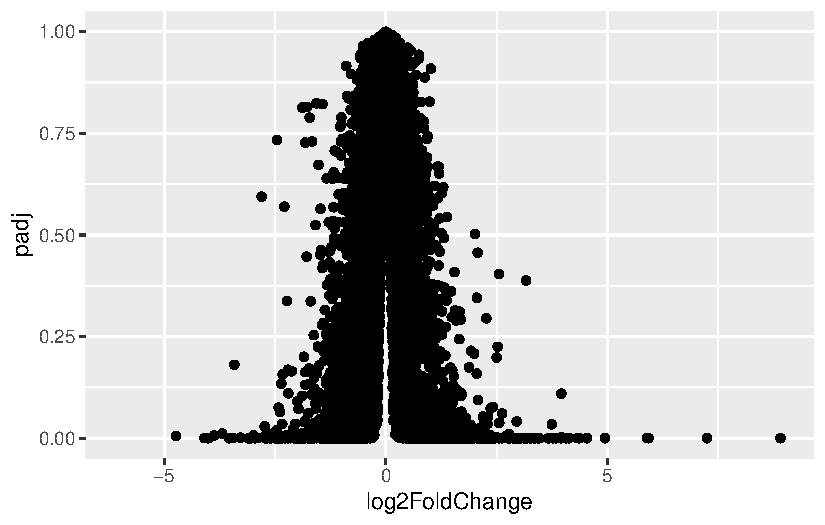
\includegraphics[keepaspectratio]{CLASS-13-WK-6-THURSDAY_files/figure-pdf/unnamed-chunk-35-1.pdf}}

\begin{Shaded}
\begin{Highlighting}[]
\FunctionTok{ggplot}\NormalTok{(res) }\SpecialCharTok{+}
  \FunctionTok{aes}\NormalTok{(log2FoldChange, }\SpecialCharTok{{-}}\FunctionTok{log}\NormalTok{(padj)) }\SpecialCharTok{+} \FunctionTok{geom\_point}\NormalTok{() }\SpecialCharTok{+} 
  \FunctionTok{geom\_vline}\NormalTok{(}\AttributeTok{xintercept =}\SpecialCharTok{{-}}\DecValTok{2}\NormalTok{, }\AttributeTok{col=}\StringTok{"red"}\NormalTok{) }\SpecialCharTok{+}
  \FunctionTok{geom\_vline}\NormalTok{(}\AttributeTok{xintercept =}\DecValTok{2}\NormalTok{, }\AttributeTok{col=}\StringTok{"red"}\NormalTok{) }\SpecialCharTok{+}
  \FunctionTok{geom\_hline}\NormalTok{(}\AttributeTok{yintercept =}\SpecialCharTok{{-}}\FunctionTok{log}\NormalTok{(}\FloatTok{0.05}\NormalTok{), }\AttributeTok{col=}\StringTok{"red"}\NormalTok{)}
\end{Highlighting}
\end{Shaded}

\begin{verbatim}
Warning: Removed 23549 rows containing missing values or values outside the scale range
(`geom_point()`).
\end{verbatim}

\pandocbounded{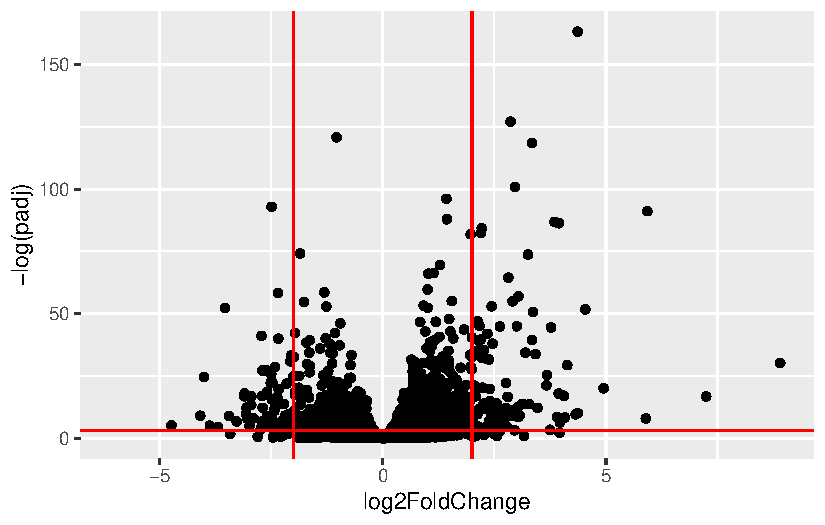
\includegraphics[keepaspectratio]{CLASS-13-WK-6-THURSDAY_files/figure-pdf/unnamed-chunk-36-1.pdf}}

\subsection{Save our results so far}\label{save-our-results-so-far}

\begin{Shaded}
\begin{Highlighting}[]
\FunctionTok{write.csv}\NormalTok{(res, }\AttributeTok{file=}\StringTok{"my\_results.csv"}\NormalTok{)}
\end{Highlighting}
\end{Shaded}

\begin{Shaded}
\begin{Highlighting}[]
\FunctionTok{ggplot}\NormalTok{(res) }\SpecialCharTok{+}
  \FunctionTok{aes}\NormalTok{(log2FoldChange, }\SpecialCharTok{{-}}\FunctionTok{log}\NormalTok{(padj), }
    \AttributeTok{color =}\NormalTok{ padj }\SpecialCharTok{\textless{}} \FloatTok{0.05} \SpecialCharTok{\&} \FunctionTok{abs}\NormalTok{(log2FoldChange) }\SpecialCharTok{\textgreater{}} \DecValTok{2}\NormalTok{) }\SpecialCharTok{+}
  \FunctionTok{geom\_point}\NormalTok{() }\SpecialCharTok{+}
  \FunctionTok{geom\_vline}\NormalTok{(}\AttributeTok{xintercept =}\SpecialCharTok{{-}}\DecValTok{2}\NormalTok{, }\AttributeTok{col=}\StringTok{"red"}\NormalTok{) }\SpecialCharTok{+}
  \FunctionTok{geom\_vline}\NormalTok{(}\AttributeTok{xintercept =}\DecValTok{2}\NormalTok{, }\AttributeTok{col=}\StringTok{"red"}\NormalTok{) }\SpecialCharTok{+}
  \FunctionTok{geom\_hline}\NormalTok{(}\AttributeTok{yintercept =}\SpecialCharTok{{-}}\FunctionTok{log}\NormalTok{(}\FloatTok{0.05}\NormalTok{), }\AttributeTok{col=}\StringTok{"red"}\NormalTok{)}\SpecialCharTok{+}
  \FunctionTok{scale\_color\_manual}\NormalTok{(}
    \AttributeTok{values =} \FunctionTok{c}\NormalTok{( }\StringTok{"TRUE"} \OtherTok{=} \StringTok{"orange"}\NormalTok{),}
    
\NormalTok{  )}
\end{Highlighting}
\end{Shaded}

\begin{verbatim}
Warning: Removed 23549 rows containing missing values or values outside the scale range
(`geom_point()`).
\end{verbatim}

\pandocbounded{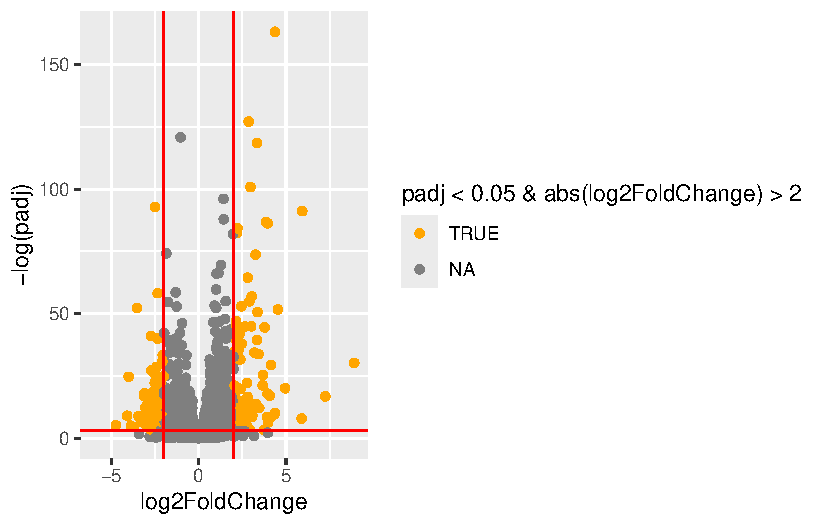
\includegraphics[keepaspectratio]{CLASS-13-WK-6-THURSDAY_files/figure-pdf/unnamed-chunk-38-1.pdf}}




\end{document}
